%%
% This is an Overleaf template for presentations
% using the TUM Corporate Desing https://www.tum.de/cd
%
% For further details on how to use the template, take a look at our
% GitLab repository and browse through our test documents
% https://gitlab.lrz.de/latex4ei/tum-templates.
%
% The tumbeamer class is based on the beamer class.
% If you need further customization please consult the beamer class guide
% https://ctan.org/pkg/beamer.
% Additional class options are passed down to the base class.
%
% If you encounter any bugs or undesired behaviour, please raise an issue
% in our GitLab repository
% https://gitlab.lrz.de/latex4ei/tum-templates/issues
% and provide a description and minimal working example of your problem.
%%

\PassOptionsToClass{onlytextwidth}{beamer}

\documentclass[
  german,            % define the document language (english, german)
  aspectratio=169,    % define the aspect ratio (169, 43)
  % handout=2on1,       % create handout with multiple slides (2on1, 4on1)
  % partpage=false,     % insert page at beginning of parts (true, false)
  % sectionpage=true,   % insert page at beginning of sections (true, false)
]{tumbeamer}


% load additional packages
\usepackage{tikz}
\usepackage{circuitikz}
\usepackage{url}
\usepackage{hyperref}
\usepackage{pgf}
\usepackage{pgfplots}
\usepackage{babel}[ngerman]
\usepackage{csquotes}[autostyle]
\usepackage[useregional]{datetime2}
\usepackage{float}
\usepackage{graphicx}
\usepackage{amsmath}
\usepackage{xcolor}
\usepackage[cache=true]{minted}
\usemintedstyle{borland}
\usepackage{listings}
\usepackage{tikz-timing}


% tikz  
\usetikzlibrary{fit, matrix, calc, arrows, arrows.meta, positioning, patterns, patterns.meta, bending, overlay-beamer-styles, shapes, shapes.geometric, shapes.misc, backgrounds}

% https://tex.stackexchange.com/a/7045
\newcommand*\circled[1]{\tikz[baseline=(char.base)]{
		\node[shape=circle,draw,inner sep=2pt, font=\scriptsize] (char) {#1};}}

\newcommand*\colorcirc[1]{\tikz[baseline=(char.base)]{
		\node[shape=circle,fill=#1,inner sep=2pt] {};}}

\newcommand\n[1]{\mkern1mu\overline{\mkern-1mu#1}}

% requires circuitikz >= 1.1.0
% for distros with older distributions, install TeX Live manually
% instead of using your package manager
% see: https://tug.org/texlive/quickinstall.html
\ctikzset{logic ports=ieee}

% minted
\setminted{
	fontsize=\small, 
	frame=none,
	breaklines=true,
}

\captionsetup{labelformat=empty}

% image path
\graphicspath{ {./resources/} }

% beamer
\setbeamercolor{footnote}{fg=black}
\setbeamercolor{footnote mark}{fg=black}
\renewcommand{\thempfootnote}{\arabic{mpfootnote}}

% presentation metadata
\title{Übung 07: Sequentielle \\Schaltungen}
\subtitle{Einführung in die Rechnerarchitektur}
\author{Niklas Ladurner}

\institute{\theChairName\\\theDepartmentName\\\theUniversityName}
\date{\DTMdisplaydate{2025}{11}{28}{-1}}

\footline{\insertauthor~|~\insertshorttitle~|~\insertshortdate}


% macro to configure the style of the presentation
\TUMbeamersetup{
  title page = TUM tower,         % style of the title page
  part page = TUM toc,            % style of part pages
  section page = TUM toc,         % style of section pages
  content page = TUM more space,  % style of normal content pages
  tower scale = 1.0,              % scaling factor of TUM tower (if used)
  headline = TUM threeliner,      % which variation of headline to use
  footline = TUM default,         % which variation of footline to use
  % configure on which pages headlines and footlines should be printed
  headline on = {title page},
  footline on = {every page, title page=false},
}

\begin{document}

\maketitle

\begin{frame}[c]{Feedback}{}
	\begin{columns}[c]
		\begin{column}{0.5\textwidth}
			\begin{center}
				\LARGE  \href{https://t1p.de/era2526}{t1p.de/era2526}\\
				
\includegraphics[height=0.5\textheight]{feedback_qr.pdf}
			\end{center}
		\end{column}
		\begin{column}{0.5\textwidth}
			\begin{center}
				\LARGE  \href{https://home.in.tum.de/~ladu/}{home.in.tum.de/\string~ladu/}\\
				\includegraphics[height=0.5\textheight]{website_qr.pdf}
			\end{center}
		\end{column}
	\end{columns}
\end{frame}

\begin{frame}[c, fragile]{}{}
	\begin{center}
		\LARGE  Keine Garantie für die Richtigkeit der Tutorfolien.

		\Large Bei Unklarheiten/Unstimmigkeiten haben VL/ZÜ-Folien recht!
	\end{center}
\end{frame}

\begin{frame}[fragile, c]{Sequentielle Schaltungen}
	\begin{columns}[c]
		\begin{column}{0.6\textwidth}
			\begin{itemize}
				\item \textbf{kombinatorische} Schaltungen: zustandsfrei, Ausgänge nur abhängig von Eingängen. \\ $\rightarrow$ z.B.: H06, Addierer, Multiplizierer
				\item \textbf{sequentielle} Schaltungen: zustandsbehaftet, Ausgänge wirken über Rückkopplung auf Schaltung ein!\\ $\rightarrow$ z.B.: Zähler, Speicher, Statusautomaten
			\end{itemize}
		\end{column}
		\begin{column}{0.4\textwidth}
			\begin{center}
				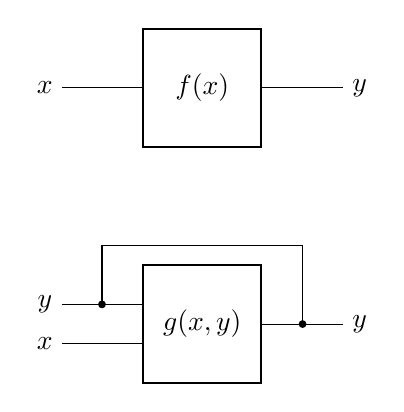
\begin{tikzpicture}[comp/.style={rectangle, draw=black, thick, minimum size=1.5cm}]
					\node[comp] (n1) {$f(x)$};
					\node[left of=n1, xshift = -1cm] (n1l) {$x$};
					\node[right of=n1, xshift = 1cm] (n1r) {$y$};
					\draw (n1l) -- (n1.west);
					\draw (n1.east) -- (n1r);

					\node[comp] (n2) [below of=n1, yshift=-2cm] {$g(x, y)$};
					\node[left of=n2, xshift=-1cm, yshift=-0.25cm] (n2l) {$x$};
					\node[left of=n2, xshift=-1cm, yshift=0.25cm] (n2lu) {$y$};
					\node[right of=n2, xshift=1cm] (n2r) {$y$};

					\draw (n2l) -- (n2l -| n2.west) node (n2ml) {};
					\draw (n2lu) -- (n2lu -| n2.west) node[midway, fill=black, circle, inner sep=1pt] (n2mlu) {};
					\draw (n2.east) -- (n2r) node[midway, fill=black, circle, inner sep=1pt] (n2mr) {};

					\node[above of=n2mr] (n2ru) {};
					\draw (n2mlu.center) |-  (n2ru.center);
					\draw (n2mr.center) -- (n2ru.center);
				\end{tikzpicture}
			\end{center}
		\end{column}
	\end{columns}
\end{frame}

\begin{frame}[c]{Latches und Flipflops\footnote{Die Definition ist hier tatsächlich ein wenig ungenau: Es gibt taktflanken- und pegelgesteuerte Flipflops, letztere werden aber im englischsprachigen Raum meist Latches genannt.}}{}
	\begin{columns}[c]
		\begin{column}{0.5\textwidth}
			\centering  \textbf{SR-Latch}\\
			\begin{itemize}
				\item  pegelgesteuert
				\item \textbf{S}et, \textbf{R}eset
				\item \enquote{verbotener} Zustand $(1,1)$, Ausgang abhängig von Implementierung
			\end{itemize}
			\vspace{0.1cm}
			\begin{center}
				\begin{circuitikz}
					\node[flipflop SR] (sr) {};
					\node[right of=sr, xshift=2cm] (arr) {
						$\displaystyle
							\begin{array}{|c|c|c|}
								\hline
								S & R & Q                 \\
								\hline
								0 & 0 & Q_{\textrm{prev}} \\
								0 & 1 & 0                 \\
								1 & 0 & 1                 \\
								1 & 1 & ?                 \\
								\hline
							\end{array}
						$};
				\end{circuitikz}
			\end{center}
		\end{column}
		\begin{column}{0.5\textwidth}
			\centering \textbf{D-Flipflop}\\
			\begin{itemize}
				\item (positiv) taktflankengesteuert
				\item Bei fallender Flanke bleibt Zustand gespeichert, bei steigender
				      Flanke wird $D$ übernommen.
			\end{itemize}
			\vspace{0.2cm}
			\begin{center}
				\begin{circuitikz}
					\node[flipflop D] (dff) {};
					\node[right of=dff, xshift=2cm] (arr) {
						$\displaystyle
							\begin{array}{|c|c|c|}
								\hline
								CLK                            & D & Q                 \\
								\hline
								\footnotesize{\texttiming{HL}} & 0 & Q_{\textrm{prev}} \\
								\footnotesize{\texttiming{HL}} & 1 & Q_{\textrm{prev}} \\
								\footnotesize{\texttiming{LH}} & 0 & 0                 \\
								\footnotesize{\texttiming{LH}} & 1 & 1                 \\
								\hline
							\end{array}
						$};
				\end{circuitikz}
			\end{center}
		\end{column}
	\end{columns}
\end{frame}


\begin{frame}[c, fragile]{}{}
	\begin{center}
		\LARGE Fragen?
	\end{center}
\end{frame}


\begin{frame}[c, fragile]{Links}{}
	\begin{itemize}
		 \item Zulip: \href{https://zulip.in.tum.de/#narrow/channel/3255-ERA-Tutorium-.E2.80.93-Mi-1600-3}{\enquote{ERA Tutorium -- Mi-1600-3}}
		bzw. \href{https://zulip.in.tum.de/#narrow/channel/3264-ERA-Tutorium-.E2.80.93-Fr-1500-1}{\enquote{ERA Tutorium -- Fr-1500-1}}
		\item \href{https://www.moodle.tum.de/course/view.php?id=111440}{ERA-Moodle-Kurs}
		\item \href{https://artemis.tum.de/courses/516}{ERA-Artemis-Kurs}
		\item \href{https://www.elektronik-kompendium.de/sites/dig/0209301.htm}{Elektronik-Kompendium zu Flipflops}
		\item \href{https://github.com/hneemann/Digital}{Repository: Digital}
	\end{itemize}
\end{frame}

\maketitle

\end{document}
